\documentclass[notes]{subfiles}
\begin{document}
	\addcontentsline{toc}{section}{1.11 - Cubic Functions \& Models}
	\refstepcounter{section}
	\fancyhead[RO,LE]{\bfseries  \large \nameref{cs111}} 
	\fancyhead[LO,RE]{\bfseries \currentname}
	\fancyfoot[C]{{}}
	\fancyfoot[RO,LE]{\large \thepage}	%Footer on Right \thepage is pagenumber
	\fancyfoot[LO,RE]{\large Chapter 1.11}


\section*{Cubic Functions \& Models}\label{cs111}
	\subsection*{Cubic Models}
		\begin{figure}[h!]
		\fbox{
			\begin{minipage}{1in}
			\centering
			$\underline{a > 0}$\\
				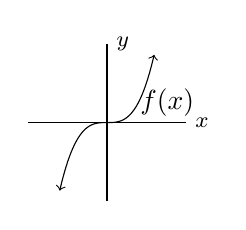
\begin{tikzpicture}[x = .5cm, y = .5cm]
					\draw (-2,0)--(2,0) node[right] {\footnotesize $x$}; %x-axis 
					\draw (0,-2)--(0,2) node[right] {\footnotesize $y$}; %y-axis
					\draw[<->, smooth, samples = 100, domain = -1.2:1.2] plot (\x, {(\x)^3});	
					\draw (.6,.5) node[right] {$f(x)$};
				\end{tikzpicture}	
			\end{minipage}
			\begin{minipage}{2in}
				\begin{itemize}
					\item $\ds \lim_{x\to\infty} f(x) =$ \showto{ins}{\fbox{$ \infty$}}\showto{st}{}
					\item $\ds \lim_{x\to -\infty} f(x) =$ \showto{ins}{\fbox{$-\infty$}}\showto{st}{}
					\item $f$ is increasing, decreasing, then increasing
					\item $f$ is concave down then up 
				\end{itemize}
			\end{minipage}
			}
		\fbox{
		\begin{minipage}{1in}
			\centering
			$\underline{a < 0}$\\
				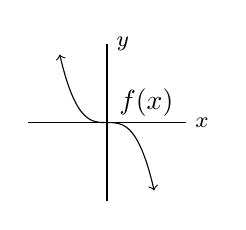
\begin{tikzpicture}[x = .5cm, y = .5cm]
					\draw (-2,0)--(2,0) node[right] {\footnotesize $x$}; %x-axis 
					\draw (0,-2)--(0,2) node[right] {\footnotesize $y$}; %y-axis
					\draw[<->, smooth, samples = 100, domain = -1.2:1.2] plot (\x, {-(\x)^3});	
					\draw (1,.5) node {$f(x)$};
				\end{tikzpicture}
		\end{minipage}
		\begin{minipage}{2in}
			\begin{itemize}
				\item $\ds \lim_{x\to\infty} f(x) =$ \showto{ins}{\fbox{$ -\infty$}}\showto{st}{}
				\item $\ds \lim_{x\to -\infty} f(x) =$ \showto{ins}{\fbox{$\infty$}}\showto{st}{}
				\item $f$ is decreasing, increasing, then decreasing
				\item $f$ is concave up then down
			\end{itemize}
		\end{minipage}
		}
		\end{figure} 

	\subsection*{Examples}
		\begin{ex} A car company's profit on SUV's is given below.  
			\begin{center}
				{\renewcommand{\arraystretch}{1.2}
				\begin{tabular}{|c||c|c|c|c|c|c|c|}\hline
					\textbf{SUV's sold} (in millions) & 10 & 20 & 30 & 40 & 50 & 60 & 70\\ \hline
					\textbf{Profit} (in trillion dollars) & 0.9 & 3.1 & 4.3 & 5.2 & 5.8 & 6.4 & 6.9\\ \hline 
				\end{tabular}		
				}
			\end{center}
			\begin{enumerate}[(a)]
				\item Use the scatterplot to determine the best model for the data.  Give two reasons for your choice.
					\vs{1}
				\item Write the complete model.
					\vs{1}
				\item Find the profit when 37 million SUV's are sold.  Write a sentence of interpretation for your answer.
					\vs{1}
			\end{enumerate}
		\end{ex}
			\newpage

		\begin{ex} A manufacturing company recorded the production of toys when a certain amount of capital is invested in the production run.
			\begin{center}
				{\renewcommand{\arraystretch}{1.2}
				\begin{tabular}{|c||c|c|c|c|c|c|}\hline
					\textbf{Capital Invested} (in  million dollars) & 6 & 18 & 24 & 30 & 42 & 48\\ \hline
					\textbf{Units Produced} (in billions)& 19 & 38 & 42 & 45 & 60 & 77\\ \hline 
				\end{tabular}
				}
			\end{center}
			\begin{enumerate}[(a)]
				\item Use the scatterplot to determine the best model for the data.  Give two reasons for your choice.
					\vs{1}
				\item Write the complete model.
					\vs{1}
				\item Find the capital needed to produce 50 billion units.  Write a sentence interpreting your answer.
					\vs{1}
			\end{enumerate}
		\end{ex}

	\clearpage
\end{document}